\section{カスタムコレクションの構築}

Clojureのコレクションがどれもあなたの問題に適していない場合、あなた自身でロールバックする必要があるかもしれません。標準のコレクションと同様に、カスタム・コレクションはClojureコア・ライブラリでシームレスに使用できます。カスタム・コレクションを構築するには、Clojureが内部で使用するtraitインタフェースを実装するためにdeftypeを使用することが必要です。

\subsection{コレクションの特徴}

Clojureが使用できるコレクションを構築したい場合、Clojureがコレクションとどのように相互作用するかをより深く理解する必要があります。コレクションとシーケンスライブラリは、Clojureに含まれる特定の実装ではなく、主要な抽象化を定義する特質の一般的なセットに基づいています。Clojureのコレクション特質は、Javaインタフェースを使用して内部的に実装されています。

述語関数は、コレクション実装上のClojureコレクションの特徴の存在を検出するためにClojureで提供されます。述語関数は質問をし、ブール値の答えを返しますが、Clojureでは慣例的に名前に末尾の\texttt{?}をつけます。

Clojureの述語コレクション関数には、以下のようなものがあります。


\begin{itemize}
\item \texttt{counted?}--コレクションは一定時間内に数えることができるか?
\item \texttt{sequential?}--値が特定のトラバース可能な順序で格納されているか?
\item \texttt{associative?}--コレクションはキーと値の間の関連性を保存しているか?
\item \texttt{reversible?}--コレクションは可逆的か?
\item \texttt{sorted?}--コレクションはソートされた順序で管理されているか?
\end{itemize}

これらの特質は、以下のJavaインタフェースに対応している。\texttt{Counted}、Sequential、\texttt{Associative}、\texttt{Reversible}、\texttt{Sorted}です。その他の内部インターフェースは、コアコレクションインターフェースの構造や、パブリックコレクション関数の下で使われる主要なメソッドを定義している。

カスタムコレクションを構築するとき、実装したいClojure関数から、その関数をサポートするためにコレクションに必要な実装のJavaインタフェースまで、逆算する必要があります。

この図は、Clojure関数(右の列)からJavaメソッド(左の列)へのマッピングを提供します。各インターフェースに対する述語関数は、各Javaインターフェース名の下に記載されています。

\begin{figure}[h]
\centering
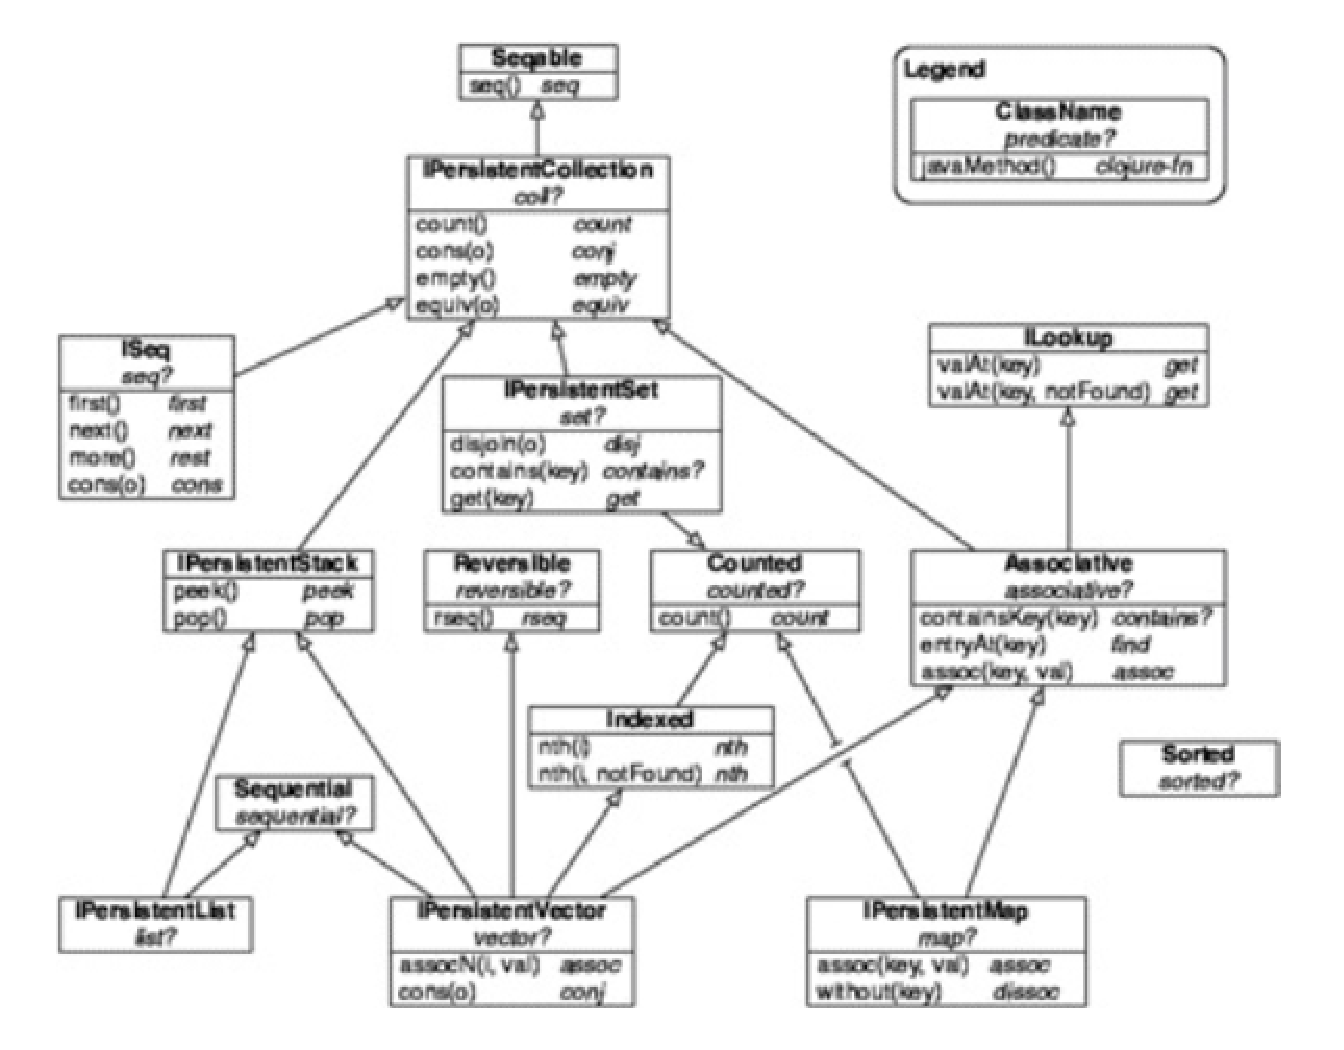
\includegraphics[width=8cm]{fig_02_002.eps}
\caption{Clojure関数とそれに対応するJavaメソッド}
\end{figure}

Clojureで意図した使用方法とマッピング図を用いて、目的を満たすカスタムコレクションを構築する方法を見てみましょう。

\subsection{deftypeでコレクションを作成する}

まず、このコレクションが何をする必要があるのかを考えてみましょう。a と b と呼ぶ 2 つの値を保持するカスタム \texttt{Pair} クラスを実装するつもりです。\texttt{Pair} 型は \texttt{seq}、\texttt{count}、\texttt{nth}、および \texttt{get} で動作するようにしたいと思います。図を見てみると、\texttt{Seqable}、\texttt{Counted}、\texttt{Indexed}、\texttt{ILookup}を実装する必要があることがわかります。

カスタムデータ構造を実装するには、\texttt{deftype}マクロを使用します。
これは\texttt{defrecord}に似ているが、より多くの機能を提供し、マップとの組み込みの類似性は少ない。例えば、\texttt{deftype}は\texttt{record}と同じように型とコンストラクタ関数を取得しますが、自動的にマップのように動作するわけではありません。\texttt{deftype}では、必要であればマップのように振舞うために適切なインタフェースを実装するのは我々の責任である。型はまた、他のClojure構成要素では利用できない、mutableフィールドやunsynchronizedフィールドのような特殊な機能のサポートを持っています。

\texttt{Pair}が\texttt{deftype}としてどのように見えるか見てみましょう。

\begin{lstlisting}[numbers=none]
(ns ch2.pair
  (import [clojure.lang Counted Indexed ILookup Seqable]))

(deftype Pair [a b]
  Seqable
  (seq [_] (seq [a b]))

  Counted
  (count [_] 2)

  Indexed
  (nth [_ i]
    (case i
      0 a
      1 b
      (throw (IllegalArgumentException.))))
  (nth [this i _] (nth this i))

  ILookup
  (valAt [_ k _]
    (case k
      0 a
      1 b
      (throw (IllegalArgumentException.))))
  (valAt [this k] (.valAt this k nil)))
\end{lstlisting}

\texttt{deftype}の内部では、実装される各インターフェースをリストアップし、次にメソッドの実装を提供します。

これでREPLから\texttt{Pair}型を利用することができるようになりました。

\begin{lstlisting}[numbers=none]
user> (use 'ch2.pair)
nil
user> (def p (->Pair :a :b))
#'user/p
user> (seq p)
(:a :b)
user> (count p)
2
user> (nth p 1)
:b
user> (get p 0)
:a
user> p
#object[ch2.pair.Pair 0x39b4cec7 "ch2.pair.Pair@39b4cec7"]
\end{lstlisting}

\texttt{p}を直接見ようとするまではうまくいっていたのですが、これから修正します。

\subsection{型のカスタム表示}

先ほど見たように、型にはクラス名と識別子を含むあらかじめ定義された表示フォーマットがあります。私たちの型の表示形式には、インスタンスデータが含まれるようにしたいのです。リーダーはClojure内部のコンポーネントで、文字列を読み込んでClojureデータを返します。理想的には、リーダーによって読むことができるフォームで私たちの型を表示したいです -- これはリテラル値として私たちに完全なラウンドトリップ能力を与えます。

表示装置は、カスタムプリンターを供給するフックを定義するマルチメソッドを持つオープンシステムです。考慮すべきは、\texttt{print-method}(ユーザのために表示するときに呼び出される)と\texttt{print-dup}(リーダーのために表示するときに呼び出される)の2つのフックである。例えば、Clojure文字列は、\texttt{print-method}では周囲の引用符なしで表示されますが、 \texttt{print-dup}では周囲の引用符で表示されます。

私たちの目的のために、私たちはどちらの場合でも同じようにペアタイプを表示したいので、単に\texttt{print-method}を呼び出すために\texttt{print-dup}を実装することにします。

\begin{lstlisting}[numbers=none]
(defmethod print-method Pair
  [pair ^Writer w]
  (.write w "#ch2.pair.Pair")
  (print-method (vec (seq pair)) w))

(defmethod print-dup Pair
  [pair w]
  (print-method pair w))
\end{lstlisting}

そのため、今回のプリンターでは、\texttt{Pair}データをベクターに変換し、既存のベクター用\texttt{print-method}に対応させることで簡略化しています。試してみましょう。

\begin{lstlisting}[numbers=none]
user> (use 'ch2.pair.print)
nil
user> (->Pair 1 2)
#ch2.pair.Pair[1 2]
user> #ch2.pair.Pair[3 4]
#ch2.pair.Pair[3 4]
\end{lstlisting}

Clojureリーダーはこの形式を使用してJavaオブジェクトを構築するため、今回表示する構文は特別に選択されました。フォーマットは\tex{#class\[args\]}です。前のコードでは、コンストラクタ・クラスの構文を REPL に置くと、リーダーはそれを \texttt{Pair} オブジェクトに読み込んで、プリンタは私たちの \texttt{print-method} プリンタを使用して結果のオブジェクトを表示します。

